%Die Geschichte Pythons wird hier erl�utert. Woraus hat sich Python entwickelt, was war die Motivation?  Weiters eine kurze Untersuchung zur Relevanz Pythons in Kombination mit Informatikunterricht mit Hilfe eines Vergleichs einer Google-Suche aus dem Jahre 2002 und 2006.

Ihren Namen verdankt die Programmiersprache Python der britischen Comedy-Gruppe Monty Python, nicht der gleichnamigen Schlangenart, wenngleich diese auch zu einem wesentlichen Bestandteil der Python \CI\ geworden ist.

Pythons Erfinder und momentaner Hauptbetreuer ist Guido van Rossum. Python basiert auf ABC, einer Programmiersprache, die in den achtziger Jahren verwendet wird. 1989 beginnt Van Rossum mit der Entwicklung von Python am \CWI\/\footnote{http://www.cwi.nl/} in Amsterdam. Das Ziel ist, die H�rden, die ABC an der Weiterverbreitung hindern, zu �berwinden. ABC ist wie Pascal: eine gute Lehrsprache f�r den Unterricht, aber in der Industrie nicht zu gebrauchen. Ein Grund ist Unflexibilit�t, wenn es um Skalierbarkeit geht.
So wird Python von Grund auf f�r den Einsatz in der Ausbildung an Lehranstalten konzipiert. Hinzu kommen mehr fortgeschrittene M�glichkeiten zur Softwareentwicklung, eine Standardbibliothek voller Erweiterungen und die leichte Ankn�pfbarkeit an andere Programmiersprachen (vor allem C), damit Python auch au�erhalb des Unterrichts Verwendung finden kann.\cite{python:teachingscientific}

\begin{figure}[h]
	\centering
	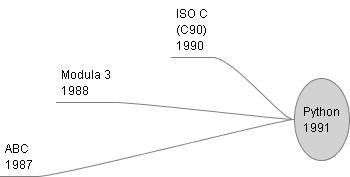
\includegraphics[scale=0.8]{graphics/history.jpg}
	\caption{Einfl�sse anderer Sprachen auf Python}
	\label{fig:history_python}
\end{figure}

Abbildung \ref{fig:history_python} zeigt eine kompakte �bersicht zur Entwicklung Pythons. Eine detaillierte, historische �bersicht zur Entstehung von Programmiersprachen im Allgemeinen ist auf \cite{python:pix} zu finden.

Python wird 1991 ver�ffentlicht; die Entwicklung der ersten Version geht bis Python 1.6.1. Oktober 2000 wird Python 2.0 freigegeben, zum Zeitpunkt dieser Arbeit ist Python in Version 2.5 aktuell, welche seit September 2006 zur Verf�gung steht. Momentan wird an Version 3.0 (Py3K, Python 3000) entwickelt, die in einer \emph{Alpha} Version 2007 erwartet wird\footnote{Python 3000, Google Tech Talk, Guido van Rossum, 2006}.

Diese Arbeit greift nun den Versuch auf, die Popularit�t Pythons anhand einer Google Suche zu messen. Das ist keine sehr wissenschaftliche Messung, spiegelt aber doch eine gewisse Relevanz und vor allem deren Ver�nderung in den letzten Jahren, in der weltweit gr��ten Suchmaschine wider. Basis der Untersuchung sind die Ergebnisse aus dem Jahr 2002 von \cite{python:teachingscientific}:

\begin{table}[h]
	\centering
	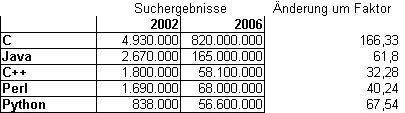
\includegraphics[scale=0.75]{graphics/google1.jpg}
	\caption[Google Vergleich 1]{Google-Suche: {\tt Platzhalter-Sprache AND ( language OR code OR program)}. Zugriff auf http://www.google.com/ am 22.10.2006.}
	\label{fig:google1}
\end{table}

Tabelle \ref{fig:google1} stellt die Ergebnisse einer Anfrage an die Suchmaschine Google dar. Dabei wird die urspr�ngliche Anfrage von \cite{python:teachingscientific} aus dem Jahr 2002 mit der gleichen - nur zeitlich aktuelleren - Anfrage verglichen. Wie zu erkennen ist, ist die Anzahl der Treffer immens in die H�he geschnellt. Das kann in erster Linie durch die technologische und inhaltliche Entwicklung der Suchmaschine begr�ndet werden, wie auch durch die Relevanz der einzelnen Suchanfragen.
\\Die hohe Trefferanzahl der Sprache C ist mit Vorsicht zu genie�en, da angenommen werden kann, dass hier einige Treffer zu C++ mitgerechnet werden. Trotzdem steht C ungeschlagen an der Spitze dieser Auswertung, was auch nicht weiter verwunderlich ist. Nach wie vor wird C in der Systemprogrammierung verwendet, Schnittstellen zu Anwendungsprogrammen sind typischerweise ebenso in C implementiert. Ein C-Compiler exisitiert f�r eine Vielzahl an Plattformen. Gerade im rasant gewachsenen Embedded Systems Bereich ist C quasi Standard.
\\Die anderen Programmiersprachen sind interessant zu beobachten, wobei Python im Vergleich zu 2002 das gr��te Wachstum verbuchen kann und sich im Gesamtvergleich mit Anwendungsentwicklungssprachen wie C++ oder Java durchaus messen kann. Im Vergleich der Skriptsprachen hat Perl vor Python die h�here Trefferanzahl.

\begin{table}[h]
	\centering
	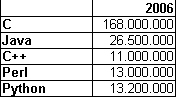
\includegraphics[scale=0.75]{graphics/google2.jpg}
	\caption[Google Vergleich 2]{Google-Suche: {\tt Platzhalter-Sprache AND ( (language OR code OR programm) AND ( education OR teaching))}. Zugriff auf http://www.google.com/ am 22.10.2006.}
	\label{fig:google2}
\end{table}

Die Daten in Tabelle \ref{fig:google1} sind sehr allgemein und umfassen mehr als die gew�nschte Thematik dieser Arbeit. Aus diesem Grund wird mit Tabelle \ref{fig:google2} die Suchanfrage leicht abge�ndert und damit konkretisiert: wie relevant sind die genannten Programmiersprachen im Unterricht? W�hrend Tabelle \ref{fig:google1} die Ver�nderung im Laufe der letzen Jahre darstellt, zeigt Tabelle \ref{fig:google2} den Status quo.
%TODO ? {\color{red} eventuell verweis auf \ref{kapitel:Programmiersprachen}}

Weiterf�hrende Literatur zu Python: \cite{python:website}, \cite{python:bytesofpython}, \cite{python:thinkCS}, 			\cite{python:programming_python}, \cite{python:cookbook}, \cite{python:diveinto}.
